\section{Prototipos}
\label{seccion-prototipos}
En la presente sección, se muestran los diferentes prototipos desarrollados durante la escritura de esta memoria. Los prototipos serán detallados utilizando una tabla resumen del mismo, la cual incluye, los Objetivos del prototipo, una Descripción, los requisitos funcionales y no funcionales que aborda el prototipo.  Se incluyen las capturas del trabajo realizado, análisis y conclusión del avance .

%En esta sección se muestran los prototipos desarrollados. Cada prototipo cuenta con una tabla para exponer el objetivo de éste, los requerimientos que aborda, imágenes del trabajo realizado y una conclusión sobre el avance del proyecto.

\subsection{Primer prototipo: Activación de motores}
\label{primer-prototipo}
Este primer prototipo tiene como principal objetivo establecer las bases necesarias para conectar de OpenGlove con un dispositivo Android y establecer una comunicación básica. Para ello se utiliza la documentación oficial de Android sobre las conexiones bluetooth \footnote{Documentación oficial android: \url{https://developer.android.com/guide/topics/connectivity/bluetooth}}, permitiendo en primera instancia la obtención de dispositivos vinculados y la conexión con alguno de los mismos. No es necesaria la modificación de código cargado en la placa arduino, puesto que los protocolos de comunicación (mensajes) ya han sido establecidos con anterioridad. Por tanto se procede a hacer uso de la API en Java de bajo nivel desarrollada por Monsalve (2015). El prototipo se resume en la Tabla \ref{table:protype-01}.


\begin{table}[H]
\centering
\caption{Primer prototipo \\ Fuente: elaboración propia (2018).}
\label{table:prototype-01}
\begin{tabular}{|l|l|}
\hline
\textbf{ID del prototipo} & \textbf{P001}                                                                                                                                                                                                                                                                                                                                                                                                                      \\ \hline
Nombre                    & Activación de motores.                                                                                                                                                                                                                                                                                                                                                                                                              \\ \hline
Objetivos                 & \begin{tabular}[c]{@{}l@{}}Verificar la correcta activación de motores en una aplicación \\ de Android nativo, utilizando las APIs de bajo nivel disponibles.\end{tabular}                                                                                                                                                                                                                                                         \\ \hline
Descripción               & \begin{tabular}[c]{@{}l@{}}El primer prototipo desarrollado hace uso de la API de bajo nivel\\ de Java desarrollada por Monsalve (2015), sumándose modificaciones\\ realizadas para establecer la conexión en Android. De esta manera,\\ se obtiene un prototipo capaz de establecer una conexión bluetooth\\ con dispositivos previamente vinculados, permitiendo activar y \\ desactivar un motor de manera remota.\end{tabular} \\ \hline
Requisitos funcionales    & RF 000                                                                                                                                                                                                                                                                                                                                                                                                                             \\ \hline
Requisitos no funcionales & RNF 000                                                                                                                                                                                                                                                                                                                                                                                                                            \\ \hline
\end{tabular}
\end{table}

Para lograr el objetivo propuesto, luego obtener los dispositivos vinculados y de la conexión con el guante mediante las APIs de bluetooth de Android, se procedió a enviar mensajes bajo el protocolo establecido en el desarrollo de Monsalve (2015). Dicho de una manera más detallada se utilizó la clase \textit{Message Generator} de la API de bajo nivel y la implementación nativa en Android para la escritura serial por medio de bluetooth. La Figura \ref{fig:prototype-01} consiste en el primer prototipo que muestra el listado de los dispositivos vinculados, la posibilidad de la conexión con el dispositivo deseado, permitiendo finalmente activar y desactivar el motor seleccionado para las pruebas. Para administrar la conexión entre el dispositivos, se requiere de un hilo encargado de ello (\textit{ConnectedThread}), el cual se comunica con el hilo de la \textit{interfaz de usuario} (UI desde ahora)  mediante mensajes. En conclusión es posible realizar envio de mensajes bajo el protocolo que acepta OpenGlove desde una aplicación Android nativa en Java.

\begin{figure}[H]
  \begin{center} 
   	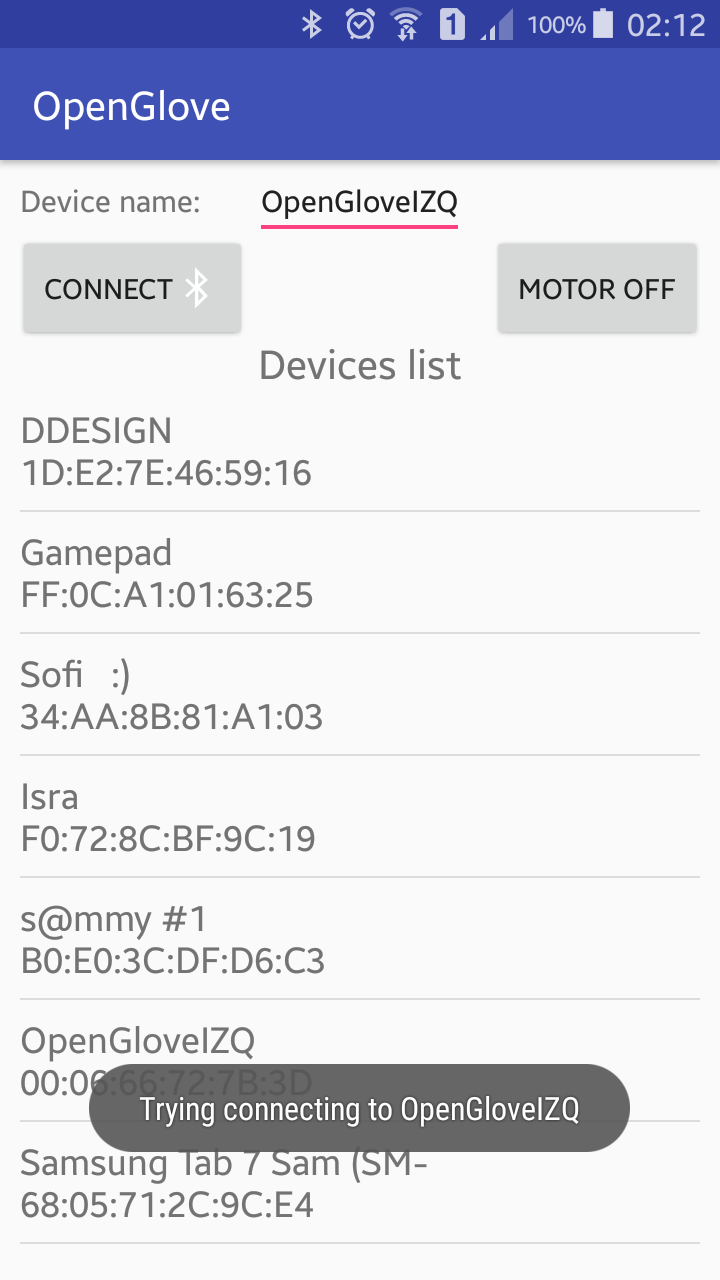
\includegraphics[width=0.3\textwidth]{images/fig-analisis-solucion/01-prototype.png} 
    \caption{Primer prototipo} 
    \label{fig:prototype-01}
  \end{center}
\end{figure}



\subsection{Segundo prototipo: Obtención de datos desde flexores}
\label{segundo-prototipo}
En el segundo prototipo se mantiene lo desarrollado previamente, añadiendo en esta iteración el soporte para los flexores. En este caso es necesaria la lectura desde el dispositivo OpenGlove. En la Tabla \ref{table:prototype-02} se muestra el resumen del prototipo ya mencionado.

\begin{table}[H]
\centering
\caption{Segundo prototipo}
\label{table:prototype-02}
\begin{tabular}{|l|l|}
\hline
\textbf{ID del prototipo} & \textbf{P002}                                                                                                                                                                                                                                                       \\ \hline
Nombre                    & Obtención de datos desde los flexores.                                                                                                                                                                                                                              \\ \hline
Objetivos                 & \begin{tabular}[c]{@{}l@{}}Verificar la correcta obtención de datos desde los flexores en \\ la aplicación de Android nativo, utilizando las APIs de bajo \\ nivel disponibles.\end{tabular}                                                                        \\ \hline
Descripción               & \begin{tabular}[c]{@{}l@{}}El segundo prototipo desarrollado agrega los métodos disponibles \\ de los flexores de la API de bajo nivel C\# hecha por Cerda (2017). \\ De esta manera, se obtiene un prototipo capaz de obtener los datos\\ del flexor.\end{tabular} \\ \hline
Requisitos funcionales    & RF 000                                                                                                                                                                                                                                                              \\ \hline
Requisitos no funcionales & RNF 000                                                                                                                                                                                                                                                             \\ \hline
\end{tabular}
\end{table}


\begin{figure}[H]
  \begin{center} 
   	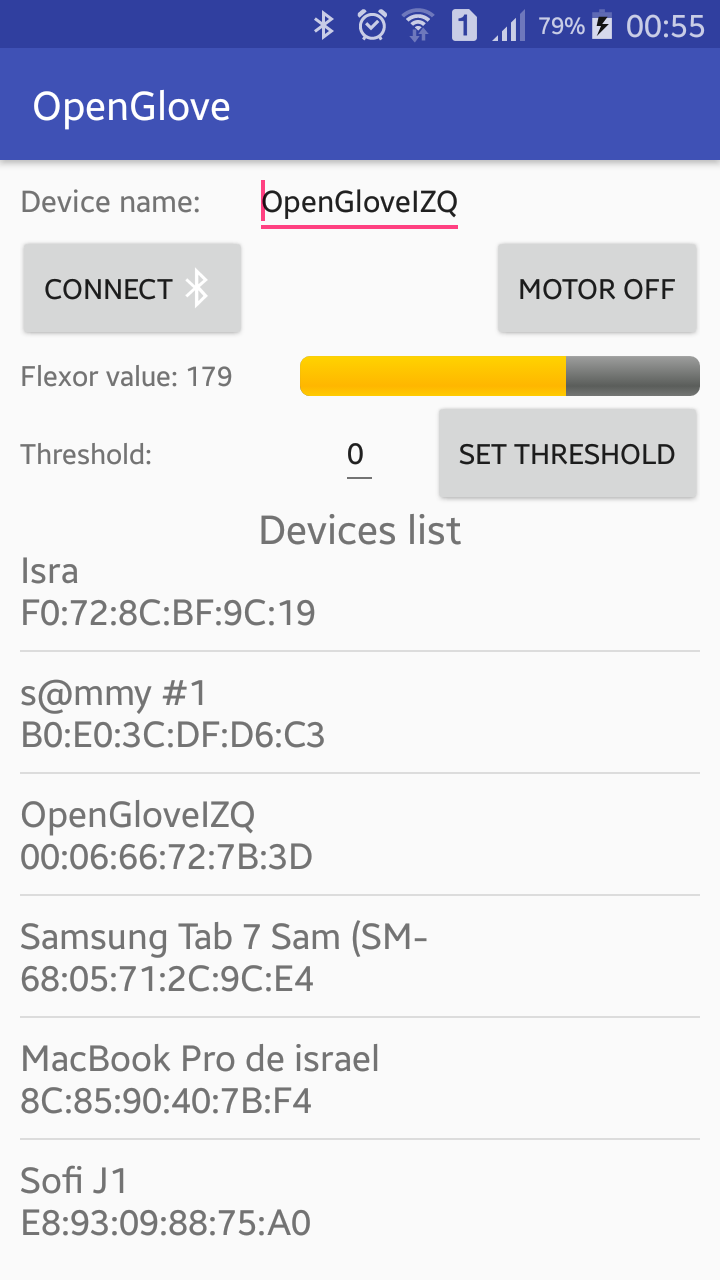
\includegraphics[width=0.3\textwidth]{images/fig-analisis-solucion/02-prototype.png} 
    \caption{Segundo prototipo} 
    \label{fig:prototype-02}
  \end{center}
\end{figure}

Para realizar la captura de datos del flexor, se obtiene valor actual del pin al cual el está conectado, esto se logra con el desarrollo de la función analogRead(pin) en Java basada en la API C\# de bajo nivel Cerda (2017). El hilo encargado de la administrar conexión (\textit{ConnectedThread}), tiene la responsabilidad de leer los mensajes desde OpenGlove y actualiza la UI enviando como un mensaje ente hilos el valor obtenido del flexor. Además se agregan las demás funciones de generación de mensajes relacionadas a los flexores en la API C\# ya mencionada. En la figura \ref{fig:prototype-02} se puede ver el estado actual del flexor el cual varia en un rango de entre 60 a 300 y 170 el valor medio del flexor sin aplicar fuerza.

\subsection{Tercer prototipo}
\label{tercer-prototipo}
% Xamarin C# prototype for cross platform use
En el segundo prototipo fue posible la activación del motor y obtener la información del flexor, permitiendo así comprobar la factibilidad de un desarrollo nativo en Android. En este tercer prototipo, se buscó dar soporte multiplataforma al proyecto, considerando la importancia de mantener umbrales de latencia, se optó por Xamarin. En concreto Xamarin.Form,  que es una tecnología de desarrollo móvil multiplataforma \footnote{Traducción libre}, el cual permite desarrollar aplicaciones nativas para Android e iOS en C\#. La tabla \ref{table:prototype-03} muestra el resumen del tercer prototipo.

\begin{table}[H]
\centering
\caption{Tercer prototipo}
\label{table:prototype-03}
\begin{tabular}{|l|l|}
\hline
\textbf{ID del prototipo} & \textbf{P003}                                                                                                                                                                                                                                                       \\ \hline
Nombre                    & Activación de motores y obtención de datos desde los flexores.                                                                                                                                                                                                                              \\ \hline
Objetivos                 & \begin{tabular}[c]{@{}l@{}}Verificar la correcta activación de motores y la obtención de \\ datos desde los flexores en la aplicación de Android nativo \\ con Xamarin.Forms, utilizando las APIs C\# de bajo nivel disponibles.\end{tabular}                                                                        \\ \hline
Descripción               & \begin{tabular}[c]{@{}l@{}}El tercer prototipo desarrollado agrega las mismas funcionalidades \\ que en el segundo prototipo.  De esta manera, se obtiene un prototipo \\ capaz de obtener los datos del flexor.\end{tabular} \\ \hline
Requisitos funcionales    & RF 000                                                                                                                                                                                                                                                              \\ \hline
Requisitos no funcionales & RNF 000                                                                                                                                                                                                                                                             \\ \hline
\end{tabular}
\end{table}



La figura \ref{fig:prototype-03} muestra el prototipo hecho en Xamarin.Forms, el cual es similar al segundo prototipo, con la diferencia en la forma de conectarse a un dispositivo bluetooth, el cual difiere en la forma de conectarse, este prototipo requiere presionar el dispositivo y aceptar el mensaje que explica el intento de conexión.


\begin{figure}[H]
  \begin{center} 
   	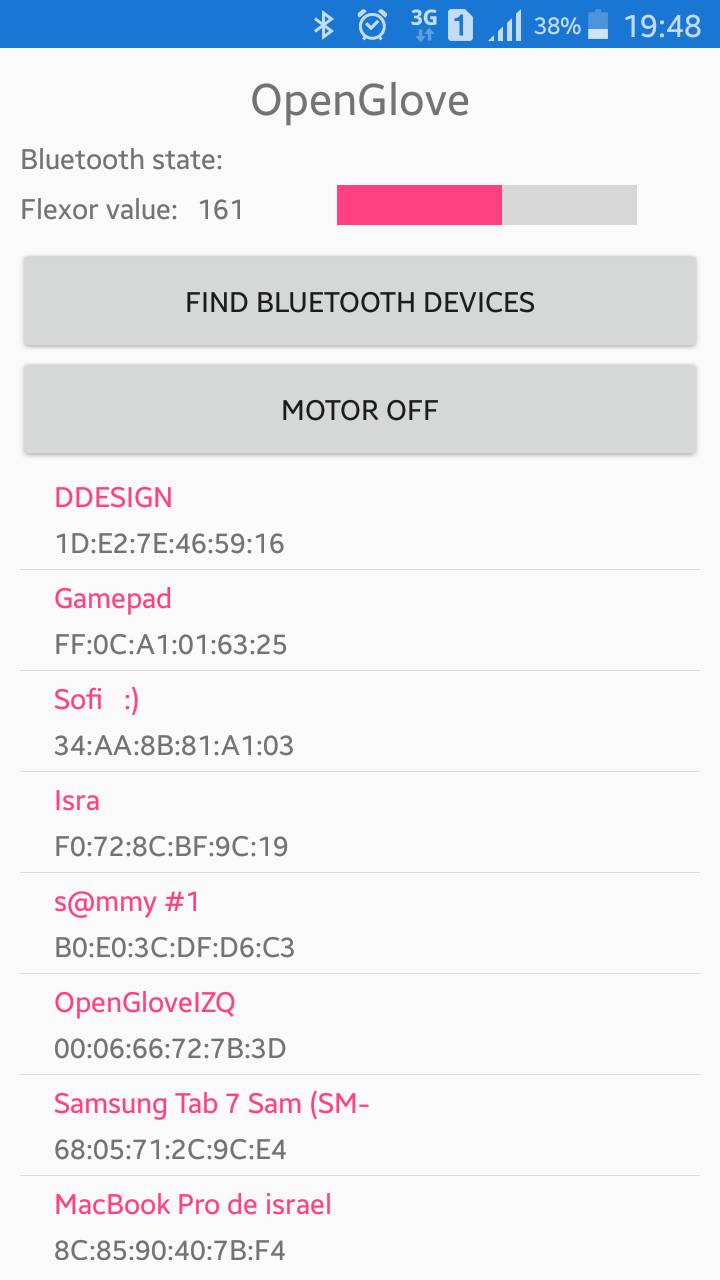
\includegraphics[width=0.3\textwidth]{images/fig-analisis-solucion/03-prototype.png} 
    \caption{Tercer prototipo} 
    \label{fig:prototype-03}
  \end{center}
\end{figure}


\subsection{Cuarto prototipo}
\label{cuarto-prototipo}
